\documentclass[preview,border=5pt]{standalone}
\usepackage{teaching}
\begin{document}

\centering

\begin{tikzpicture}[yscale=2,xscale=1,scale=0.5,inner sep=0.3mm, label distance=1.5mm]

\node(t) at (0,1) {\large $x = \dfrac{-b\pm\sqrt{b^2-4ac}}{2a}$};

\end{tikzpicture}

\end{document}